\chapter{Recursive State Estimation}

Let's assume that we are moving in an environment, we are tasked with estimating the environment and our position. We are doing something similar here as compared to multi view geometry, but recursively.

Let's say we have data upto a time $t$, and we wish to estimate the state of the system at $t+1$th instant. In most of the methods mentioned earlier, there was no time factor involved. Here, we want to use time series data to estimate the next belief state. Just as in dynamic programming, to estimate $t+2$th instant, we don't want to restart everything. In essence, we don't want to estimate the state of the system.

With recursive state estimation, we only use the new data that is incoming to estimate and do not use data till that time $t$. We assume that the information till that point has been incorporated already and we move from belief at time $t$ to belief at time $t+1$. This is very similar to the markov chain discussed in probability. This chapter will explore bayes filter, kalman filter and more. 

\section{Bayesian Filter}

Our goal is to estimate the state of the system $x$ given the observation $z$ and controls $u$. Imagine an environment filled with pillars, and as a robot moves we want to estimate the state of the system. Obviously this is important because we cannot control a robot without knowing where it is. The control is what command we give. The observation is our observation of where we are. This is very similar to the POMDP scenario where we have observations, actions and belief states. The observations can be derived from a sensor (laser range finder, GPS, etc). This can be concisely be represented as:

\begin{equation}
    bel(x_t) = P(x_t|z_{1:t},u_{1:t})
\end{equation}

Our goal is to represent this information using $x_{t-1}$.

\begin{figure}
    \centering
    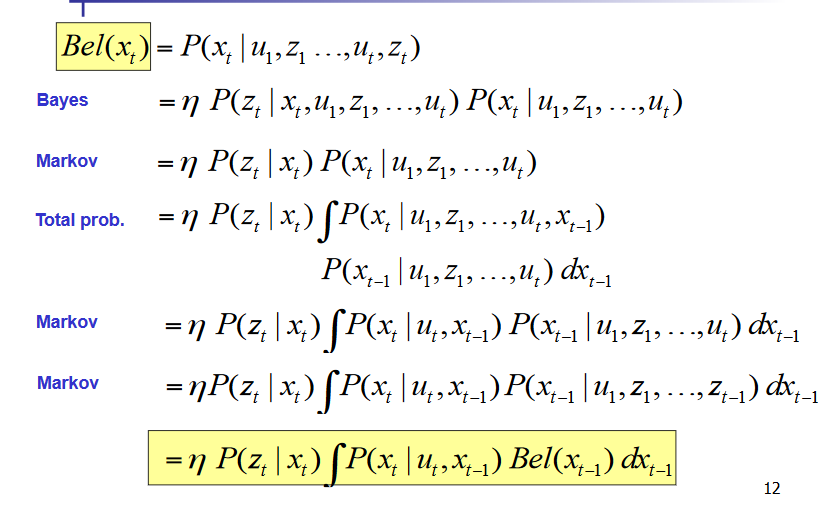
\includegraphics[width=8cm]{img/bayes-filter.png}
    \caption{Bayesian Filter Derivation}
    \label{fig:bayes_filter}
\end{figure}

\textbf{Markov Assumption}

The Markov assumption is that observation of the system at a time $t$ is only dependent on the time $t$ and not on any of the observation before it. Hence, we need not use $z_{1:t}$ and $u_{1:t}$ since we used that information already to arrive at our current state.

The bayesian filter is a framework for recursive state estimation.

\begin{equation}
    \hat{bel(x_t)} = \int p(x_t\|u_t, x_{t-1})bel(x_{t-1})dx_{t-1}
\end{equation}

After correction, we get:

\begin{equation}
    bel(x_t) = \eta p(z_t\|x_t)\hat{bel(x_t)}
\end{equation}

\section{Kalman Filter}

This is essentially a bayesian filter with gaussians - a very popular filter. We know what a gaussian is already. For a multivariate gaussian, it looks something like:

\begin{equation}
    p(x) = \frac{1}{(2\pi)^{d/2}\abs{\Sigma}^{1/2}}e^{-\frac{1}{2}(x-\mu)^t\Sigma^{-1}(x-\mu)}
\end{equation}

\begin{figure}
    \centering
    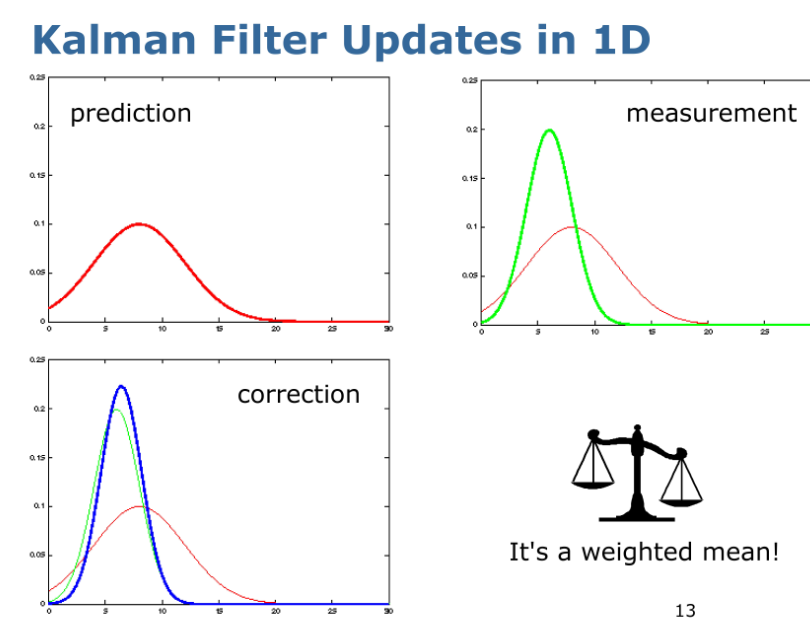
\includegraphics{img/kalman.png}
    \caption{Kalman Filter}
    \label{fig:kalman}
\end{figure}

He didn't really cover this in much detail but it uses covariance matrices and a concept called "Kalman" gain to make updates to the estimate.

\section{Extended Kalman Filters}

So far, we've only looked at linear functions. Kalman filters work with gaussian distributions and linear functions. But the world isn't that \textbf{straight} forward (badum-tus). Non linear functions needn't preserve the initial distribution and the kalman filter can BREAK. 

So, we find a hack and try to linearize our non-linear functions. This is usually done with a Taylor series expansion. For higher dimension data, note that we use jacobians to linearize the data.